% =============================================================================
% Avalia — Big Data Technologies project report
% Compile: ./build.sh   (lualatex + biber + biblatex)
% =============================================================================
\documentclass[11pt,a4paper]{article}

% ---------- Layout ----------
\usepackage[margin=2.4cm,top=2.2cm,bottom=2.4cm]{geometry}
\setlength{\parindent}{0pt}
\setlength{\parskip}{6pt}
\linespread{1.04}

% ---------- Fonts: Latin Modern + unicode-math (fixes \url math errors) ----------
\usepackage{fontspec}
\setmainfont{Latin Modern Roman}
\setmonofont{Latin Modern Mono}[Scale=0.92]
\usepackage{unicode-math}
\setmathfont{Latin Modern Math}
\usepackage{microtype}

% ---------- Color (subtle navy reserved for hyperlinks only) ----------
\usepackage{xcolor}
\definecolor{linkcol}{HTML}{1F3A5F}
\definecolor{boxfr}{gray}{0.45}
\definecolor{muted}{gray}{0.45}

% ---------- Section spacing (default LaTeX styling otherwise) ----------
\usepackage{titlesec}
\titlespacing*{\section}      {0pt}{12pt plus 2pt minus 2pt}{4pt}
\titlespacing*{\subsection}   {0pt}{8pt plus 2pt minus 2pt}{3pt}
\titlespacing*{\subsubsection}{0pt}{6pt plus 2pt minus 2pt}{2pt}

% ---------- Lists, tables, callouts ----------
\usepackage{enumitem}
\setlist{itemsep=3pt,topsep=4pt,parsep=0pt,leftmargin=1.6em}
\usepackage{booktabs,array,tabularx}
\usepackage[most]{tcolorbox}
\usepackage{float}    % provides the [H] specifier to lock floats in place
\usepackage{caption}
\captionsetup{font=small,skip=4pt}

% ---------- Float spacing ----------
\setlength{\textfloatsep}{10pt plus 2pt minus 2pt}
\setlength{\floatsep}{10pt plus 2pt minus 2pt}
\setlength{\intextsep}{10pt plus 2pt minus 2pt}
\setlength{\abovecaptionskip}{6pt}
\setlength{\belowcaptionskip}{3pt}

% ---------- TikZ ----------
\usepackage{tikz}
\usetikzlibrary{positioning,arrows.meta,calc}

% ---------- Bibliography ----------
\usepackage[
  backend=biber,
  style=apa,
  sorting=nyt,
  maxbibnames=99,
  uniquename=false,uniquelist=false
]{biblatex}
\addbibresource{references.bib}

% ---------- Hyperlinks ----------
\usepackage[colorlinks=true,linkcolor=linkcol,urlcolor=linkcol,citecolor=linkcol]{hyperref}

% ---------- Page footer ----------
\usepackage{fancyhdr}
\pagestyle{fancy}\fancyhf{}
\renewcommand{\headrulewidth}{0pt}
\renewcommand{\footrulewidth}{0pt}
\fancyfoot[C]{\thepage}

\begin{document}

% =============================================================================
% BEGIN GREGOR SECTION  — delete everything between BEGIN and END markers
% before submission.  The rest of the report is self-contained.
% =============================================================================
\thispagestyle{empty}
\vspace*{1.4cm}
\begin{center}
{\Large\bfseries Organization for Gregor}\\[3pt]
{\itshape\small Navigation aid only. Remove before submission.}
\end{center}
\vspace{10pt}

\begin{tcolorbox}[
  colback=white,colframe=boxfr,boxrule=0.4pt,arc=1pt,
  boxsep=6pt,left=12pt,right=12pt,top=10pt,bottom=10pt
]
\noindent Each rubric sub-point links to the section in the body that addresses it. Internal links are clickable in the PDF.

\medskip
\textbf{1.\ Relevance}
\begin{enumerate}
  \item \hyperref[sec:intro]{One-sentence pitch and why it qualifies as a Big Data project.}
  \item \hyperref[sec:intro]{Beneficiaries and business case.}
  \item \hyperref[sec:roadmap]{Monetisation and sustainability.}
\end{enumerate}

\textbf{2.\ Innovation}
\begin{enumerate}
  \item \hyperref[sec:differentiation]{Differentiation versus existing portals.}
  \item \hyperref[sec:forecast]{How AI and other tools were applied.}
  \item \hyperref[sec:roadmap]{Next steps to become a real business.}
\end{enumerate}

\textbf{3.\ Maturity}
\begin{enumerate}
  \item \hyperref[sec:system]{Functional prototype.}
  \item \hyperref[sec:system]{Reproducibility and access.}
  \item \hyperref[sec:limits]{Known issues.}
\end{enumerate}

\textbf{4.\ Presentation.}\ \ Slides and live demo, 20 May pitch. Out of scope for this written report.

\medskip
\noindent\textbf{Cross-cutting topics requested:}
\begin{itemize}
  \item \hyperref[sec:limits]{Cloudflare D1 100\,000-writes/day cap and why it forced Lisbon-only scope.}
  \item \hyperref[sec:data]{Full data-source list (habitacao.net, arquivo.pt, Google Trends, PORDATA, INE).}
  \item \hyperref[sec:system]{What the frontend does (seven pages and a Lisbon map).}
  \item \hyperref[sec:forecast]{How the forecast is computed.}
  \item \hyperref[sec:fivevs]{The 5\,Vs of Big Data, current state, scaled vision, growth estimates.}
\end{itemize}

\medskip
\noindent\textit{To remove: delete everything between\,\texttt{\% BEGIN GREGOR SECTION}\,and\,\texttt{\% END GREGOR SECTION} in \texttt{report.tex} and rerun \texttt{./build.sh}.}
\end{tcolorbox}

\newpage
% =============================================================================
% END GREGOR SECTION
% =============================================================================

% ---------- Title block ----------
\begin{center}
{\LARGE\bfseries Avalia: A Big Data Lens on the\\[2pt] Lisbon Real-Estate Market}\\[10pt]
{\large Daniel Freire Mendes \quad Danish Mujtaba Qureshi \quad Gregor Stefan Sonntag}\\[5pt]
\textit{Big Data Technologies}\\[3pt]
\href{https://github.com/danielfmendes/Avalia}{github.com/danielfmendes/Avalia} \quad
\href{https://avalia-frontend.pages.dev}{avalia-frontend.pages.dev}
\end{center}

\medskip
Avalia turns twelve years of Portuguese property listings, plus tourism, search, and macro signals, into parish-level intelligence and twelve-month forecasts for Lisbon.

% ---------- 1. Introduction ----------
\section{Introduction}\label{sec:intro}

Portuguese property portals (Idealista, Imovirtual, Casa Sapo) only show \emph{current} listings. No public record tracks how prices evolved per parish (\emph{freguesia}) over the last decade, and none of those portals surfaces the macro-economic and behavioural signals that move the market.

\textbf{User stories.}
\begin{itemize}
  \item As a \emph{renter or buyer}, I want decade-long price history for my parish, to negotiate from evidence.
  \item As a \emph{small landlord or agent}, I want year-on-year parish benchmarks, to price listings competitively.
  \item As a \emph{municipal planner}, I want housing-pressure indicators correlated with tourism and search, to target interventions.
\end{itemize}

\textbf{Why this is a Big Data project.} The base dataset is 2.6\,GB of raw listings ($\sim$3\,million transactions) drawn from the Portuguese web archive \emph{arquivo.pt} via the open-data project \emph{habitacao.net}. Two further sources, Google Trends and PORDATA, join it at weekly to annual cadences (Section~\ref{sec:data}). Volume, Variety, and Veracity are present from day one. Velocity and full Value are out of scope for the prototype and analysed in Section~\ref{sec:fivevs}.

% ---------- 2. System ----------
\section{System architecture and reproducibility}\label{sec:system}

Seven pages, filterable by sale type and room count, share a D3-Geo Lisbon map that drills district~$\to$~municipality~$\to$~parish:
\begin{itemize}
  \item \emph{Market Overview}: district prices, KPI cards, drill-down map.
  \item \emph{AI Predictions}: 12-month forecast per region with uncertainty bands.
  \item \emph{Signals}: price overlaid on Google Trends, \emph{dormidas}, earnings, construction.
  \item \emph{Compare}: side-by-side comparison of up to six municipalities or parishes.
  \item \emph{Rooms}: T0--T4+ bedroom-type analysis with per-room trends.
  \item \emph{Affordability}: budget slider that ranks parishes within reach.
  \item \emph{Time Machine}: monthly scrubber back to 2012, with gainers and losers.
\end{itemize}

\begin{figure}[H]
\centering
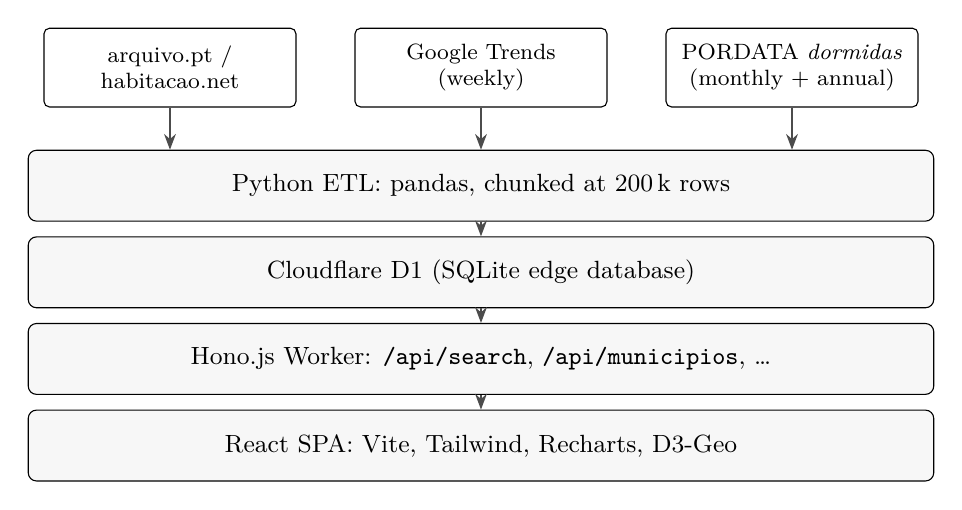
\begin{tikzpicture}[
  font=\footnotesize,
  src/.style  ={draw,rounded corners=2pt,minimum width=3.2cm,minimum height=10mm,align=center,fill=white},
  layer/.style={draw,rounded corners=3pt,minimum width=11.5cm,minimum height=9mm,align=center,fill=black!3,font=\small},
  arrow/.style={-{Stealth[length=2mm]},semithick,black!70}
]
% Three source boxes, evenly spaced and centred under the layer column (centre x = 5.65)
\node[src] (s1) at (1.7 ,0) {arquivo.pt /\\habitacao.net};
\node[src] (s2) at (5.65,0) {Google Trends\\(weekly)};
\node[src] (s3) at (9.6 ,0) {PORDATA \emph{dormidas}\\(monthly + annual)};
\node[layer] (etl) at (5.65,-1.5) {Python ETL: pandas, chunked at 200\,k rows};
\node[layer] (db)  at (5.65,-2.6) {Cloudflare D1 (SQLite edge database)};
\node[layer] (api) at (5.65,-3.7) {Hono.js Worker: \texttt{/api/search}, \texttt{/api/municipios}, \ldots};
\node[layer] (fe)  at (5.65,-4.8) {React SPA: Vite, Tailwind, Recharts, D3-Geo};
\draw[arrow] (s1.south) -- (s1.south |- etl.north);
\draw[arrow] (s2.south) -- (s2.south |- etl.north);
\draw[arrow] (s3.south) -- (s3.south |- etl.north);
\draw[arrow] (etl) -- (db);
\draw[arrow] (db)  -- (api);
\draw[arrow] (api) -- (fe);
\end{tikzpicture}
\caption{Avalia data pipeline. Three heterogeneous sources are normalised by a Python ETL into a single Cloudflare D1 schema, served by a Hono.js Worker, and consumed by a React single-page application with map-based drill-down.}
\label{fig:arch}
\end{figure}

Source code, ETL scripts, and the database schema are version-controlled in the GitHub repository, and the live demo is publicly accessible (links in the References).

% ---------- 3. Data sources ----------
\section{Data sources}\label{sec:data}

\begin{itemize}
  \item \textbf{arquivo.pt and habitacao.net.} \emph{arquivo.pt} is Portugal's web archive, with periodic snapshots of major property portals (Idealista, Imovirtual, Casa Sapo). The open-data project \emph{habitacao.net} mines those snapshots to reconstruct advertised-listings history back to 2012, exposing price, area, room count, and location for each entry.
  \item \textbf{Google Trends.} Weekly Lisbon housing-keyword search interest, used as a leading indicator. Spikes in queries like ``comprar casa'' tend to precede price moves by one or two months.
  \item \textbf{PORDATA.} Per-municipality time-series from the Francisco Manuel dos Santos Foundation. We use tourism overnights (\emph{dormidas}, monthly) as a proxy for short-term-rental pressure, plus four annual macro series: foreign workers, tourist capacity, mean monthly earnings, and completed constructions.
\end{itemize}

\renewcommand{\arraystretch}{1.18}
\begin{table}[H]
\centering
\begin{tabularx}{\linewidth}{@{}lXl@{}}
\toprule
\textbf{Source} & \textbf{Content} & \textbf{Cadence} \\
\midrule
arquivo.pt + habitacao.net & 2.6\,GB raw listings, $\sim$3\,M transactions      & historical \\
Google Trends              & Lisbon search interest                              & weekly     \\
PORDATA \emph{dormidas}    & tourism overnights per municipality                 & monthly    \\
PORDATA macro              & foreign workers, tourist capacity, mean earnings, completed constructions & annual \\
\bottomrule
\end{tabularx}
\caption{Data sources, contents, and refresh cadences.}
\label{tab:sources}
\end{table}

\nocite{arquivo,habitacao,googleTrends,PORDATA,avaliaRepo,avaliaDemo}

% ---------- 4. Forecasting ----------
\section{Forecasting model}\label{sec:forecast}\label{sec:differentiation}

For each region, the frontend takes the trailing 18 monthly averages of €/m\textsuperscript{2}, fits an ordinary-least-squares line, and projects 12 months ahead. The uncertainty band widens by 1.5\,\% per step. The model runs entirely client-side.

\textbf{What is different.} Where Idealista shows the present, Avalia shows \emph{history} (\emph{Time Machine} scrubs back to 2012) and \emph{future} (12-month projections), and overlays exogenous signals on price curves so users \emph{see} what moves the market.

\textbf{AI in the build.} Code generation throughout was AI-assisted (Claude Code), with the prompt log committed to the repository.

\textbf{Planned forecast upgrade.} The current model only extrapolates each region's own past prices, so it captures inertia but misses turning points. The next version adds Google Trends, tourism overnights, and the PORDATA macro series as predictors and fits them jointly against price, so the forecast reflects live demand and macro context, sharpening accuracy when the market accelerates or cools.

% ---------- 5. Five Vs ----------
\section{The 5\,Vs of Big Data: today and at scale}\label{sec:fivevs}

\begin{table}[H]
\centering
\renewcommand{\arraystretch}{1.32}
\begin{tabularx}{\linewidth}{@{}>{\bfseries}p{1.7cm}XX@{}}
\toprule
\textbf{V} & \textbf{Today (Lisbon prototype)} & \textbf{At scale (national + live)} \\
\midrule
Volume   & 2.6\,GB raw, aggregated to 65\,k rows over the Lisbon AML          & $\sim$10\,GB raw, $\sim$250\,k aggregated, live ingestion adds 0.5--1\,M rows/yr \\
Velocity & Batch reload only                                                  & A managed streaming ingestion pipeline pulling 500--1\,000 listings/day, with hourly aggregate refresh \\
Variety  & Four external sources (search, tourism, demographics, construction) plus core listings & + transit/walkability, school ratings, mortgage rates, weather, EU energy certificates \\
Veracity & Weighted means, chunked dedup, type coercion                       & Cross-portal reconciliation, anomaly detection, listing-survival modelling \\
Value    & Yield calculator, affordability heatmap, signal overlay            & Personalised recommendations, probabilistic forecasts, municipal-pressure index \\
\bottomrule
\end{tabularx}
\caption{Mapping of the 5\,Vs of Big Data onto the current prototype and the production-scale system.}
\label{tab:fivevs}
\end{table}

\textbf{Growth estimate.} Portuguese real-estate transactions run at $\sim$150--200\,k purchases per year nationally. Combining the historical \emph{arquivo.pt} extract with continuous portal scraping pushes the corpus from today's 65\,k rows to roughly \textbf{1.5\,M after three years}, which a higher tier of the same managed database absorbs without changing the architecture. Every gap in Table~\ref{tab:fivevs} is bridged by a known technology, not new research.

% ---------- 6. Discussion ----------
\section{Discussion and conclusion}\label{sec:roadmap}

\subsection{Monetisation and roadmap}

Three revenue lines are plausible: a freemium consumer tier with a paid \emph{investor} mode, a B2B API for banks and agencies, and anonymised market reports for municipalities. Next steps: ingest the full national \emph{arquivo.pt} corpus, add daily scraping of live portals, and productionise the multivariate forecasting pipeline described in Section~\ref{sec:forecast}.

\subsection{Limitations}\label{sec:limits}

Cloudflare D1's free tier caps writes at \textbf{100\,000 rows per day} \parencite{cloudflareD1}, which is why we scoped the prototype to the eighteen Lisbon Metropolitan Area municipalities. Aggregating to month\,$\times$\,parish\,$\times$\,type\,$\times$\,rooms compresses $\sim$3\,M rows to $\sim$65\,k for Lisbon, inside the cap. The forecasting model does not yet use the available exogenous regressors, and refresh is manual.

% ---------- References ----------
\printbibliography[title={References}]

\end{document}
